\newpage
\section{Durchführung}
\label{sec:Durchführung}
Während dieses Experimentes befinden sich alle Bestandteile auf einer Schiene,
damit die relativen Abstände variiert werden können. Der gesamte Aufbau ist in
Abbildung \ref{fig:Versuchsaufbau1} abgebildet.
\begin{figure}[htb]
  \centering
  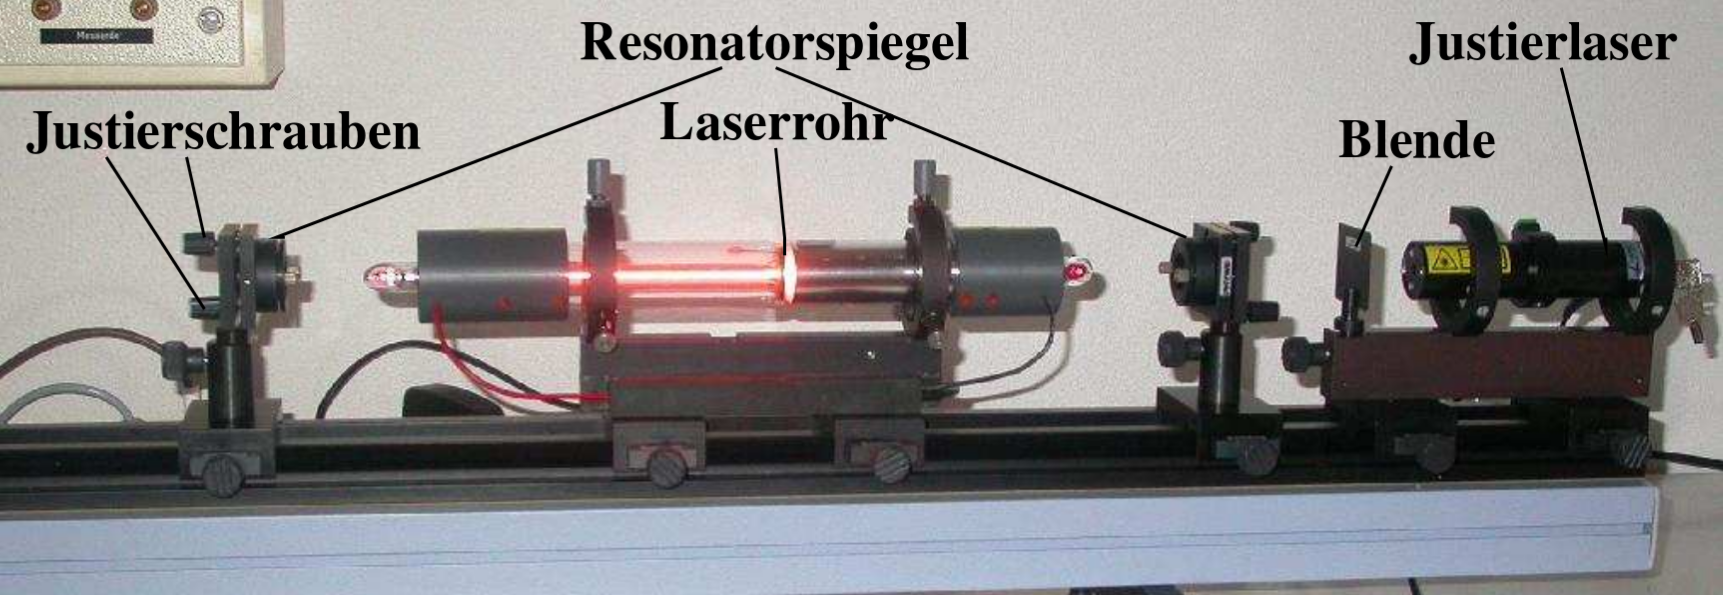
\includegraphics[width=0.8\textwidth]{content/aufbau.png}
  \caption{Aufbau eines HeNe-Lasers mit Justagelaser \cite{anleitung}.}
  \label{fig:Versuchsaufbau1}
\end{figure}
\FloatBarrier

\subsection{Justage}

Zunächst müssen die einzelnen Bestandteile justiert werden.
Zu diesem Zweck wird ein weiterer Laser und zwei Lochblenden verwendet.
Um die notwendige Gasentladung zu erhalten, wird eine Hochspannung an das Laserrohr
angelegt. Um nun den Laser zum lasern zu bringen, werden die konfokalen
Resonatorspiegel mit Justierschrauben an Spiegeln und laserrohr so eingestellt,
dass alle optischen Achsen aufeinander liegen. Dabei ist eine Photodiode zu
Intensitätsmessung hinter dem Laser angebracht.

\subsection{Bestimmung der Wellenlänge}
Um die Wellenlänge
des erzeugten Lasers zu messen, wird ein optisches Gitter verwendet.
Zur Vermessung des entstehenden Interferenzbildes wird hinter das Gitter ein Schirm
gestellt, an dem die Abstände zwischen den auftretenden Interferrenzmaxima vermessen
werden können. Aus diesen Abständen und aus der Messung des Abstandes zwischen Schirm und Gitter
kann die Wellenlänge durch
\begin{equation}
  \lambda = \frac{g\cdot\sin(\phi)}{n},\ \ \phi = \arctan\left(\frac{d_\text{n}}{L}\right),\  n\in\mathds{N}
  \label{eqn:welle}
\end{equation}
berechnet werden. Hierbei ist $g$ die Gitterkonstante, $d_\text{n}$ der Abstand zwischen Hauptmaxima
und $n$-ten Maximum und $L$ der Abstand zwischen Gitter und Schirm.

\subsection{Unteruchung der TEM-Moden}
Zur Untersuchung der TEM-Moden wird eine defokussierende Linse hinter den Laser gestellt.
So wird der Strahl des Lasers verbreitert und die Untersuchung erleichtert.
Um die Photodiode senkrecht zu der Strahlenachse verschieben zu können, wird eine
Mikrometerschraube verwendet. Durch Verschieben der Photodiode kann
die Intensität in Abhängigkeit des Achsenabstands bestimmt werden.

Die Grundmode ist ohne Einsatz von Blenden und Gittern zu untersuchen.
Die $I_{01}$-Mode wird vermessen,
indem ein Wolframdraht zwischen den Resonatorspiegeln positioniert wird,
dass die Grundmode unterdrückt wird.
Die $I_{01}$-Mode besitzt eine Nullstelle bei $r = 0$
und wird ebenfalls durch Verschieben der Photodiode senkrecht zur Strahlenachse
untersucht.

\subsection{Untersuchung der Polarisation}
Zur Überprüfung der Polarisation der Lasers sind an den Ausgängen des
Laserrohrs Brewster-Fenster angebracht. Brewster-Fenster sind gläsernde Platten, die einen
zur optischen Achse eingestellten Brewsterwinkel besitzen. Als Brewsterwinkel wird
jener Winkel bezeichnet, bei dem nach den Fresnelschen Formel kein parallel zur
Einfallsebene polarisertes Licht reflektiert wird. Zudem wird das senkrecht zur
Einfallsebene polarisierte Licht durch Reflexion stark unterdrückt. Somit ist der
verbleibende Lichtstrahl linear polarisiert.

Zur Untersuchung dieser Begebenheit wird das Gesetz von Malus verwendet, welches
die Intensität des Strahls hinter dem Polasisationsfilter beschreibt. Mit
den konstanten Parametern $I_0$ und $\phi_0$ wird in Abhängigkeit des Drehwinkels
$\phi$ die verbleibende Intensität berechnet durch
\begin{equation}
  I(\phi) = I_0\sin^2(\phi+\phi_0).
\end{equation}

\subsection{Überprüfung der Stabilitätsbedingung}
Damit die Richtigkeit der Stabilitätsbedingung überprüft werden kann, wird die
variierte Resonatorlänge $L$ gegen den Photostrom aufgezeichnet. Hierzu
werden ein gekrümmter Spiegel $r=\SI{1.4}{\metre}$ und ein ebener Spiegel verwendet.
Bei jeder Variation der Resonatorlänge ist dabei die Justage neu durchzuführen,
um den Photostrom zu maximieren.
